% !TEX TS-program = LuaLaTeX
\documentclass[11pt,compress,xcolor=x11names,UTF8]{beamer}
\usetheme{Boadilla}
\usecolortheme{seahorse}
\useinnertheme[shadow]{rounded}  
\useoutertheme[subsection=false]{smoothbars}
\usecolortheme{spruce}
\usecolortheme[named=SpringGreen4]{structure}
\usefonttheme{structurebold}
\useinnertheme{circles}
\usecolortheme{rose}
\usepackage{pifont}
\usepackage{academicons}
\usepackage{fontawesome}
\usepackage{iitem}
\setbeamertemplate{itemize item}{\ding{108}}
\setbeamertemplate{itemize subitem}{\ding{109}}
\setbeamertemplate{navigation symbols}{}
\setbeamercovered{transparent}  
\renewcommand\appendixname{附录}
\renewcommand\abstractname{摘要}
\graphicspath{{figure/}} % 图片路径
\usepackage{calligra} % Thank you
\usepackage{ctex} % 加入中文
%\setCJKsansfont{Noto Sans CJK SC}
\setsansfont{Lato} % Lato Roboto Fira Sans
\usepackage{makecell}
\newcommand{\tabincell}[2]{\begin{tabular}{@{}#1@{}}#2\end{tabular}}
\usepackage{url}					
\usepackage{natbib} % 参考文献
%\title[Spatial Generalized Linear Mixed Models]{Spatial Generalized Linear Mixed Models with Application to Prevalence Mapping}
\title{中期考核答辩}
%\subtitle{奖助金申请答辩}
\author[赵荣]{学生:赵荣 \and 导师:王为 } % \\ 专业:统计学 \\ 方向:数据分析与统计计算
\institute[中山大学]{物理学院 \and 粒子物理与原子核物理\and } % 理学院\\
\date[\today]{\includegraphics[width=.5\textwidth]{logo}}

\begin{document}

\maketitle

\begin{frame}{Outline}
\tableofcontents
\end{frame}

\section{个人简介}

%\subsection{研究意义}

\begin{frame}{自我介绍}
%\textsf{例} \textbf{例}  \textit{例} 
% \texttt{例}  % 调出仿宋字体了
\begin{enumerate}
\item 2017级博士生
\item 专业:粒子物理与原子核物理
\item 导师:王为教授
\item \alert{主要研究方向:江门中微子实验}
\end{enumerate}

\end{frame}
%
%\begin{frame}{Introduction}
%\citet{Diggle2002}
%\begin{itemize}
%\item First item in the list
%\item Second item
%\item and so on
%\begin{itemize}
%\item First item in the list
%\item Second item
%\item and so on
%\end{itemize}
%\end{itemize}
%


\section{课程学习}
%%%%%%%%%%%%%%%%%%%%%%%%%%%%%%%%%%%%%%%%%%%%%%%%%%%%%
\begin{frame}{课程成绩}
2017.09-2018.06 课程学习阶段:
\begin{tabular}{ccccc}
\hline
课程 & 核电子学& 高能物理数据分析&粒子物理&高能物理简介\\ \hline
成绩 & 94 & 94 &93 &90\\ \hline
\end{tabular}
\begin{tabular}{cccc}
课程 & \tabincell{c}{粒子物理与核物理\\实验方法}& 第一外国语&中国马克思主义与当代\\ \hline
成绩 & 85 & 84 &83 \\ \hline
\end{tabular}
\end{frame}


\section{学术活动}
%%%%%%%%%%%%%%%%%%%%%%%%%%%%%%%%%%%%%%%%%%%%%%%%%%%%%%%%%%%%%%%%%%%%
\begin{frame}{学术会议}
\begin{itemize}
\item (2018.01 南京大学)第11届江门中微子实验合作组会\\
	\alert{“LED光谱分布和对PMT探测效率测量的影响”}
\end{itemize}
\begin{figure}
\centering
\includegraphics[width=0.88\textwidth]{led} % 单图
\end{figure}
\end{frame}
%%%%%%%%%%%%%%%%%%%%%%%%%%%%%%%%%%%%%%%%%%%%%%%%%%%%%%%%%%%%%%%%
%\begin{frame}{学术活动}
%\begin{itemize}
%\item (2018.03 费米国家加速器实验室)Excellence in Detector and Instrumentation Technologies\\
%	\alert{介绍江门中微子实验以及光电倍增管探测器}
%\end{itemize}
%\begin{figure}
%\centering
%\includegraphics[width=0.61\textwidth]{fermi} % 单图
%\end{figure}
%\end{frame}
%%%%%%%%%%%%%%%%%%%%%%%%%%%%%%%%%%%%%%%%%%%%%%%%%%%%%%%%%%%%%%%%
\begin{frame}{学术活动}
\begin{itemize}
\item (2018.03 费米国家加速器实验室)Excellence in Detector and Instrumentation Technologies\\
	\alert{操作各种探测器以及分析数据,获得卓越探测器完成奖}
\end{itemize}
\begin{figure}
\centering
\includegraphics[width=0.81\textwidth]{edit} % 单图
\end{figure}
\end{frame}
%%%%%%%%%%%%%%%%%%%%%%%%%%%%%%%%%%%%%%%%%%%%%%%%%%%%%%%%%%%%%%%%
\begin{frame}{学术活动}
\begin{itemize}
\item (2018.05 武汉大学)江门中微子实验离线软件探讨会\\
	\alert{学习交流江门中微子实验的离线软件开发和使用}
\end{itemize}
\begin{figure}
\centering
\includegraphics[width=0.45\textwidth]{wuhan} % 单图
\includegraphics[width=0.35\textwidth]{junosoft} % 单图
\end{figure}
\end{frame}
%%%%%%%%%%%%%%%%%%%%%%%%%%%%%%%%%%%%%%%%%%%%%%%%%%%%%%%%%%%%%%%%%%%%
\begin{frame}{学术会议}
\begin{itemize}
\item (2018.07 中国科学院高能物理研究所)第12届江门中微子实验合作组会\\
	\alert{“PMT测试数据分析和结果”}
\end{itemize}
\begin{figure}
\centering
\includegraphics[width=0.88\textwidth]{pmt} % 单图
\end{figure}
\end{frame}
\section{科研工作}
%%%%%%%%%%%%%%%%%%%%%%%%%%%%%%%%%%%%%%%%%%%%%%%%%%%%%%%%%%%%%%%%
\begin{frame}{学术活动}
\begin{itemize}
\item (2018.02 中山市)江门中微子光电倍增管测试站\\
	\alert{光电倍增管批量测试值班}
\end{itemize}
\begin{figure}
\centering
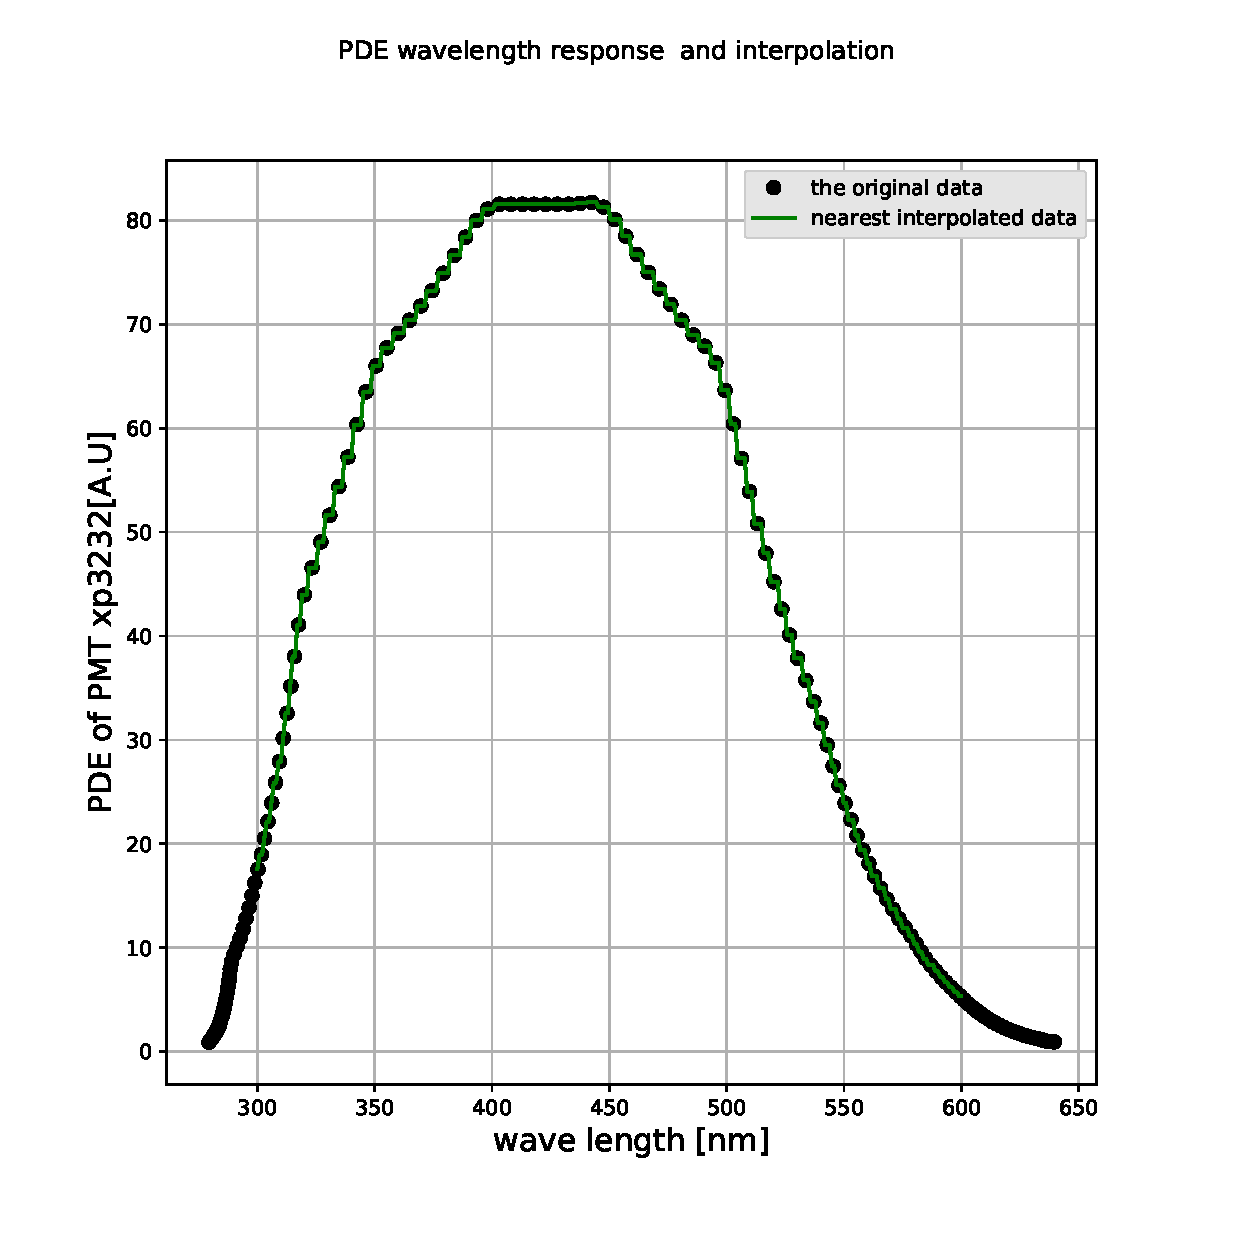
\includegraphics[width=0.451\textwidth]{pmttest} % 单图
\includegraphics[width=0.451\textwidth]{pmts} % 单图
\end{figure}
\end{frame}
%%%%%%%%%%%%%%%%%%%%%%%%%%%%%%%%%%%%%%%%%%%%%%%%%%%%%%%%%%%%%%%%
\begin{frame}{软件开发--光电倍增管批量测试数据分析软件}

江门中微子实验需要测试大约20000只光电倍增管,获得每只探测器的工作参数。
\vspace{.6cm}
\hline

\begin{itemize}
\item 基于C++ 和ROOT开发
\item 快速处理PMT测试原始数据
\item 提供详尽的测试结果分析和数据输出
\item 改进传统参数评估算法
\item 协助值班员快速查找解决硬件问题
\item 光电倍增管整体参数评估
\end{itemize}

\hline

\end{frame}
%%%%%%%%%%%%%%%%%%%%%%%%%%%%%%%%%%%%%%%%%%%%%%%%%%%%%%%%%%%%%%%%
\begin{frame}{软件开发--光电倍增管批量测试数据分析软件}
\vspace{-1cm}
\begin{figure}
\centering
\includegraphics[width=1.0451\textwidth]{pmtsoftware} % 单图
\end{figure}
\end{frame}

\section{总结}

\begin{frame}
\centering {\zihao{0} \color{red} \calligra{Thank You}}

\end{frame}


%\begin{frame}[allowframebreaks]
%\frametitle{References}
%\scriptsize
%\bibliographystyle{authordate1}
%\bibliography{R-GLMM-pkgs}
%\end{frame}

\appendix

\section*{附录}

%\begin{frame}{Softwares and Tools}

%\includegraphics[width=.2\textwidth]{software/r}\qquad
%\includegraphics[width=.16\textwidth]{software/stan} \\ 
%\includegraphics[width=.45\textwidth]{software/bioconductor}
%\includegraphics[width=.45\textwidth]{software/PyMC3} 

%\end{frame}
%% OpenBUGS  WinBUGS  JAGS
% library(R2OpenBUGS) # 2017-2-20 version 3.2-3.2
% library(R2WinBUGS) # 2015-07-29 version 2.1-21
% library(rjags) # 2016-02-19 version 4-6
% library(BRugs) # OpenBUGS 2017-06-26  version 0.9-0
% library(glmmBUGS) # Generalised Linear Mixed Models with BUGS and JAGS 2016-09-22 version 2.4.0
% library(R2jags) # Using R to Run 'JAGS'  2015-08-23	 version 0.5-7

% network
	% diagram DiagrammeR DiagrammeRsvg
 % library(help=graph)

 % library(help=Rgraphviz)
 % library(help=igraph)


%\begin{frame}{Ack}
%\begin{itemize}
%\item[\faGithub] \href{https://github.com/Cloud2016}{Cloud2016} \faAt Github
%\item[\aiOverleaf] \href{https://www.overleaf.com/}{Xiangyun} \faAt Overleaf
%\item[\aiarXiv] \href{https://arxiv.org/}{arXiv}
%\end{itemize}
%\end{frame}

\end{document} 


